\section{批量评价}
\label{sec:bo-batch}

到现在为止，算法一次只运行一个试验，等结果回来再决定下一个。如果手上有两台机器，就可以同时跑两个。于是要问：多个试验同时运行时，候选应当怎样选，尚未返回的试验又该如何处理？

并行带来的好处和代价都很具体。图~\ref{fig:bo-parallel-timeline}比较了完成四次评价的三种方式。(a)一台机器逐个运行，每次选点都能用上之前全部结果，总时长最长。(b)两台机器同步批量运行，时长减半，但第$2$次评价没有用上第$1$次的结果。(c)两台机器异步运行，耗时不等，一台空出来就立刻派新试验，此时另一台上的试验还没有结果。

\begin{BookInlineFigure}
 \centering
 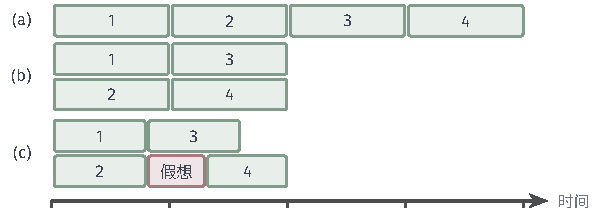
\includegraphics[width=102mm]{figures/05-optimization/05-stochastic-optimization/tikz/bo-parallel-timeline/figure.pdf}
 \caption{四次评价的三种安排，横轴是时间，每个绿框是一次评价，数字是选点顺序。(a)串行。(b)两台机器的同步批量。(c)异步，两台机器上的评价耗时不等，第$3$次选点时第$2$次评价还在运行，第$2$次评价后段的红框表示这段时间里结果尚未返回，第$3$次选点的计算对它使用假想结果，它不是观测。}
 \label{fig:bo-parallel-timeline}
\end{BookInlineFigure}

\subsection{联合选点}
\label{sec:bo-joint-batch}

一次选$q$个点时，最容易想到的做法是取单点采集分数最高的$q$个位置。问题在于这$q$个点常常挤在一个峰上。图~\ref{fig:bo-batch-joint}是贯穿例$t=4$时、在$0.25$网格上选两点的结果：单点EI最高的两点是$x=6.25$和$x=6$（黄方块），它们几乎重复。

应当衡量的是整批的价值。无噪声时，一批候选$\bm{x}_1',\ldots,\bm{x}_q'$的批量期望改进（q-EI）是
\begin{equation}
 \mathrm{qEI}_t(\bm{x}_1',\ldots,\bm{x}_q')=\mathbb{E}\Bigl[\bigl(b_t-\min_{j\leq q}F(\bm{x}_j')\bigr)_+\,\Bigm|\,\mathcal{D}_t\Bigr].
 \label{eq:bo-qei}
\end{equation}
期望对这$q$个函数值的联合后验取，所以候选点之间的相关性直接影响整批的价值。

\paragraph{相关性怎样影响整批价值}
用两个候选说清楚。设$b_t=0$，两者的后验均为$N(0,1)$，相关系数为$\rho$。单点EI都是$\phi(0)\approx0.399$，这里记$X=-F(\bm{x}_1')$，$Y=-F(\bm{x}_2')$，则
\[
 \mathrm{qEI}=\mathbb{E}\max\{0,X,Y\}.
\]

三个数$0,X,Y$从小到大排列为$U_1\leq U_2\leq U_3$。对$a,b,c$两两取最大值再求和，结果等于最大数的两倍加中间数，所以
\[
 2U_3+U_2=\max\{0,X\}+\max\{0,Y\}+\max\{X,Y\}.
\]

$(X,Y)$与$(-X,-Y)$同分布，取负号后最小的变成最大的，中间的仍是中间的，并且符号相反，所以$\mathbb{E}U_2=0$。两边取期望，再用
\[
 \mathbb{E}\max\{0,X\}=\frac1{\sqrt{2\pi}},\qquad
 \mathbb{E}\max\{X,Y\}=\sqrt{\frac{1-\rho}{\pi}},
\]
其中第二式来自$\max\{X,Y\}=(X+Y+\lvert X-Y\rvert)/2$和$X-Y\sim N(0,2(1-\rho))$，得到
\begin{equation}
 \mathrm{qEI}=\frac1{\sqrt{2\pi}}+\frac12\sqrt{\frac{1-\rho}{\pi}}.
 \label{eq:bo-qei-two}
\end{equation}

取$\rho=1,0.5,0$时，$\mathrm{qEI}$依次约为
\[
 0.399,\qquad 0.598,\qquad 0.681.
\]
两点完全相同时，第二个点没有价值，整批的价值就是单点EI；越不相关，第二个点带来的额外机会越大。但即使独立，第二个点的边际价值也小于单点EI的$0.399$，因为它和第一个点要竞争同一个“成为更好者”的位置。所以把单点分数相加不等于整批的价值。

回到贯穿例。单点EI最高的两点，整批$\mathrm{qEI}\approx0.407$，两点的单点EI之和却是$0.719$。$0.25$网格上最好的一对是$x=2.25$和$x=6.25$（绿点），整批$\mathrm{qEI}\approx0.487$，第二个点不再去挤第一个峰。

\begin{BookInlineFigure}
 \centering
 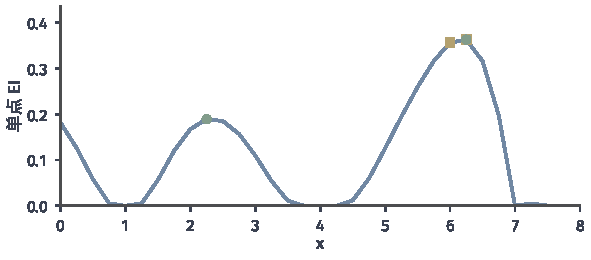
\includegraphics[width=100mm]{figures/05-optimization/05-stochastic-optimization/matplotlib/bo-batch-joint/figure.pdf}
 \caption{一次选两点。贯穿例$t=4$，$0.25$网格，蓝线是单点EI。黄方块是单点分数最高的两点（$x=6$与$x=6.25$），绿点是使$\mathrm{qEI}$最大的两点（$x=2.25$与$x=6.25$），后者由$40000$个公共后验样本估计，$x=6.25$的绿点与黄方块重合。}
 \label{fig:bo-batch-joint}
\end{BookInlineFigure}

$q$大时联合优化是$qn$维的内层问题，闭式也不再存在，通常用联合样本近似期望，再用重参数化式~\eqref{eq:bo-joint-sample}对候选位置求梯度。

\subsection{未完成的评价}
\label{sec:bo-pending}

异步运行时，一台机器空出来要立刻派新试验，而另一台上的试验还没有结果。本小节的问题是：尚未返回的试验，在选点计算中该如何对待。

忽略它们不对。忽略后下一轮的选择可能恰好与运行中的位置重复。图~\ref{fig:bo-pending-fantasy}中，若$x=6$的试验正在运行，黄线仍在$x=6$处给出高分。把运行中的位置也算作数据，就要用读数，而读数还没有。

正确做法是对可能的结果作平均。设运行中的位置为$\bm{x}_{\mathrm{p}}$，结果按当前预测分布取值，定义
\begin{equation}
 \bar\alpha_t(\bm{x})=\mathbb{E}_{y_{\mathrm{p}}}\bigl[\alpha_t\bigl(\bm{x}\mid\mathcal{D}_t\cup\{(\bm{x}_{\mathrm{p}},y_{\mathrm{p}})\}\bigr)\bigr],
 \label{eq:bo-fantasy}
\end{equation}
其中期望按$y_{\mathrm{p}}\sim N(m_t(\bm{x}_{\mathrm{p}}),s_t^2(\bm{x}_{\mathrm{p}})+\tau^2)$计算，实际常用少量抽样近似。

这里用于计算的$y_{\mathrm{p}}$称为假想结果，它不是观测，不能写进$\mathcal{D}_t$，算完就丢弃。真实结果返回后，仍须用真实读数更新后验。

看$\bm{x}_{\mathrm{p}}=6$的情形（无噪声，$t=3$）。对任何假想结果，$x=6$处的后验方差都变为零，改善量都是$0$，平均之后$\bar\alpha_3(6)=0$。图中绿线在$x=6$降到零，附近也被压低，$x=8$的分数从$0.276$降到约$0.233$，因为阈值在有些假想情形下变低了。这样下一台机器不会与运行中的试验重复。

\begin{BookInlineFigure}
 \centering
 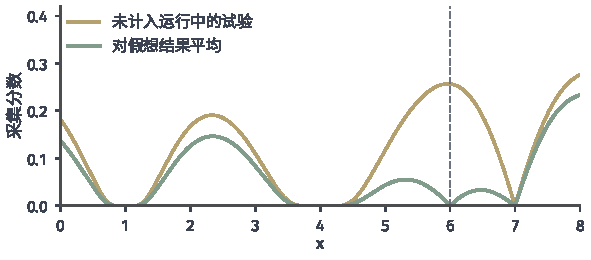
\includegraphics[width=100mm]{figures/05-optimization/05-stochastic-optimization/matplotlib/bo-pending-fantasy/figure.pdf}
 \caption{对运行中试验的处理。贯穿例$t=3$，竖虚线是运行中的位置$x=6$。黄线是不考虑运行中试验的EI，绿线是对假想结果取平均之后的EI（$201$个等分位假想读数）。绿线在$x=6$处为$0$。}
 \label{fig:bo-pending-fantasy}
\end{BookInlineFigure}
